%%% Demographic Research Pandoc Style
%%% Jonas Schöley
%%% 2019-01-25
%%% Depends on file "DemRes.bst" for custom bibliography styling.

\documentclass[10pt, twoside, parskip=half]{article}
\raggedbottom

%%%% font/encoding %%%%%%%%%%%%%%%%%%%%%%%%%%%%%%%%%%%%%%%%%%%%%%%%%%%%%%%%%%%%

\usepackage[utf8]{inputenc}          % .tex-file text encoding
\usepackage[T1]{fontenc}             % vector fonts and special chars in output
\usepackage{times}                   % Times Roman font family

%%%% maths %%%%%%%%%%%%%%%%%%%%%%%%%%%%%%%%%%%%%%%%%%%%%%%%%%%%%%%%%%%%%%%%%%%%

\usepackage{mathrsfs} % maths script fonts
\usepackage{amssymb}  % maths symbols
\usepackage{amsmath}  % various maths features

%%%% figures %%%%%%%%%%%%%%%%%%%%%%%%%%%%%%%%%%%%%%%%%%%%%%%%%%%%%%%%%%%%%%%%%%

  \usepackage{graphicx} % include external images
  % -- We will generate all images so they have a width \maxwidth. This means
  % -- that they will get their normal width if they fit onto the page, but
  % -- are scaled down if they would overflow the margins.
  \makeatletter
  \def\maxwidth{\ifdim\Gin@nat@width>\linewidth\linewidth
  \else\Gin@nat@width\fi}
  \makeatother
  \let\Oldincludegraphics\includegraphics
  \renewcommand{\includegraphics}[1]{\Oldincludegraphics[width=\maxwidth]{#1}}

%%%% captions %%%%%%%%%%%%%%%%%%%%%%%%%%%%%%%%%%%%%%%%%%%%%%%%%%%%%%%%%%%%%%%%%

\usepackage{float}      % captions above
\usepackage[hang]{caption}
\DeclareCaptionLabelSeparator{capsep}{:\hspace{1cm}}
\captionsetup[figure]{
            labelsep        = capsep,
            name            = Figure,
            font            = bf,
            labelfont       = bf,
            justification   = raggedright,
            singlelinecheck = false
}

\captionsetup[table]{
            labelsep        = capsep,
            name            = Table,
            font            = bf,
            labelfont       = bf,
            justification   = raggedright,
            singlelinecheck = false
}

% captions above
\floatstyle{plaintop}
\restylefloat{table}
\restylefloat{figure}

%%%% localization %%%%%%%%%%%%%%%%%%%%%%%%%%%%%%%%%%%%%%%%%%%%%%%%%%%%%%%%%%%%%

% babel
\usepackage[english]{babel}         % document language/localization
\usepackage[htt]{hyphenat}          % hyphenation rules

%%%% bibliography %%%%%%%%%%%%%%%%%%%%%%%%%%%%%%%%%%%%%%%%%%%%%%%%%%%%%%%%%%%%%

\usepackage{natbib}
\setcitestyle{aysep={}}
\bibliographystyle{DemRes}
\newcommand{\doi}[1]{\href{http://www.dx.doi.org/#1}{\textcolor{blue}{doi:#1}}}

%%%% layout %%%%%%%%%%%%%%%%%%%%%%%%%%%%%%%%%%%%%%%%%%%%%%%%%%%%%%%%%%%%%%%%%%%

\usepackage{geometry}
\geometry{
  paperheight = 22cm,
  paperwidth  = 17cm,
  top         = 2.54cm,
  bottom      = 2.54cm,
  inner       = 2cm,
  outer       = 2.54cm,
  footskip    = 11mm,
  headheight  = 1cm,
  headsep     = 0.75cm,
  showframe   = false
}

% change spacing
\setlength{\parskip}{0ex}
\setlength{\parindent}{.7cm}
\setlength{\bibsep}{.18cm}

% no page numbers
\pagenumbering{gobble}

% avoid orphans and widows
\widowpenalty = 10000
\clubpenalty  = 10000

% don't break footnotes
\interfootnotelinepenalty = 10000

% don't hyphenate across pages
\brokenpenalty10000\relax

% tight lists
\providecommand{\tightlist}{%
  \setlength{\itemsep}{0pt}\setlength{\parskip}{0pt}}

%%%% sections %%%%%%%%%%%%%%%%%%%%%%%%%%%%%%%%%%%%%%%%%%%%%%%%%%%%%%%%%%%%%%%%%

% spacing
\makeatletter
\renewcommand\section{\@startsection {section}{1}{\z@}%
                                   {-24pt}%
                                   {2.3ex \@plus.2ex}%
                                   {\normalfont\large\bfseries}}
\renewcommand\subsection{\@startsection{subsection}{2}{\z@}%
                                     {-24pt}%
                                     {1.5ex \@plus .2ex}%
                                     {\normalfont\normalsize\bfseries}}
\makeatother

% style
\usepackage{titlesec}
\titleformat{\section}[hang]{\raggedright\normalfont\bfseries\large}{\arabic{section}.}{1ex}{}
\titleformat{\subsection}[hang]{\raggedright\normalfont\bfseries}{\arabic{section}.\arabic{subsection}}{1ex}{}
\titleformat{\subsubsection}[hang]{\raggedright\normalfont\bfseries}{\arabic{section}.\arabic{subsection}.\arabic{subsubsection}}{1ex}{}

%%%%% footnotes %%%%%%%%%%%%%%%%%%%%%%%%%%%%%%%%%%%%%%%%%%%%%%%%%%%%%%%%%%%%%%%

% Footnotes
\usepackage[bottom]{footmisc}
\setlength{\footnotemargin}{0.6em}

% if you have code in your footnotes, the million macro march
% kind of bumps into itself.
% Pandoc, having just rendered your text into LaTeX,
% knows whether the 'variable' `verbatim-in-note` is True, and
% If it is, it asks for a  LaTeX package that solves the dilemma:

%%%% tables %%%%%%%%%%%%%%%%%%%%%%%%%%%%%%%%%%%%%%%%%%%%%%%%%%%%%%%%%%%%%%%%%%%

  \usepackage{array,longtable,booktabs,multirow}
  % -- This is needed because raggedright in table elements redefines \\:
  \newcommand{\PreserveBackslash}[1]{\let\temp=\\#1\let\\=\temp}
  \let\PBS=\PreserveBackslash
  \usepackage{etoolbox} % global table format
  \AtBeginEnvironment{tabular}{\scriptsize\sffamily}

%%%% subscripts %%%%%%%%%%%%%%%%%%%%%%%%%%%%%%%%%%%%%%%%%%%%%%%%%%%%%%%%%%%%%%%


%%%% links %%%%%%%%%%%%%%%%%%%%%%%%%%%%%%%%%%%%%%%%%%%%%%%%%%%%%%%%%%%%%%%%%%%%

\usepackage{hyperref}
\hypersetup{
  hidelinks,
  breaklinks=true,
  pdftitle={The Age-Trajectory of Infant Mortality in the United States: Parametric
Models and Generative Mechanisms}
}

%%%% misc %%%%%%%%%%%%%%%%%%%%%%%%%%%%%%%%%%%%%%%%%%%%%%%%%%%%%%%%%%%%%%%%%%%%%

% for colored links
\usepackage{xcolor}

% Footnotes:

%%%% includes %%%%%%%%%%%%%%%%%%%%%%%%%%%%%%%%%%%%%%%%%%%%%%%%%%%%%%%%%%%%%%%%%

% header_includes

%%%% title, authors %%%%%%%%%%%%%%%%%%%%%%%%%%%%%%%%%%%%%%%%%%%%%%%%%%%%%%%%%%%

  \title{\large\textbf{The Age-Trajectory of Infant Mortality in the United States: Parametric
Models and Generative Mechanisms}\vskip 0em}
\date{\vspace{-5ex}}

%%%% document %%%%%%%%%%%%%%%%%%%%%%%%%%%%%%%%%%%%%%%%%%%%%%%%%%%%%%%%%%%%%%%%%

\begin{document}

  \maketitle

\vspace*{-24pt}
\vspace*{5mm}
\setlength{\parskip}{0.5em}
\section*{Abstract}
  \noindent\textbf{BACKGROUND}\\
  While there is a consensus that the risk of death follows a Gompertz law
  over much of the adult age span, no such agreement exists about the
  parametric form of mortality at the very beginning of life with most
  literature on the topic suggesting either an exponential or various
  power-law expressions.
  \par
  \noindent\textbf{OBJECTIVE}\\
  In this paper I aim to identify the parametric shape of the infant
  mortality age-trajectory as observed in recent US birth cohorts across a
  range of social and medical strata.
  \par
  \noindent\textbf{RESULTS}\\
  Age-specific infant mortality in the US displays both power-law and
  exponential behavior and is better described by a product of those
  functions: an ``exponentially-truncated power-law''. Across all infant
  populations under consideration the age-trajectory of mortality
  following birth is initially dominated by a power-law regime and over
  the course of infancy eventually approaches an exponential decline of
  less than a 1\% reduction per additional day of age. The hazard of
  infant death varies in a highly non-proportional fashion by prematurity
  and health of the infant upon birth.
  \par
  \noindent\textbf{CONTRIBUTION}\\
  The exponentially-truncated power-law hazard is a novel tool for the
  study of infant mortality being more parsimonious than smoothing-splines
  while providing interpretable parameters and an excellent fit over a
  range of diverse populations. The transition from a power-law dominated
  neonatal mortality schedule to an exponential post-neonatal hazard has
  not been noted before and suggests an underlying shock-recovery or
  mortality selection process.
\vspace*{12pt}

\setlength{\parskip}{0ex}

\newpage

\section{Background}\label{background}

Since Benjamin Gompertz published his eponymous law of mortality for the
adult ages many suggestions have been made for a law of similar
generality describing the age pattern of infant and/or childhood
mortality. Perhaps the earliest attempt was published by
\citet{Oppermann1870} who proposed\footnote{Throughout the paper
  \(\mu(x)\) denotes the force of mortality at age \(x\).}
\(\mu(x)=ax^{-1/2}+b+cx^{1/2}\) for mortality prior to age 20. With a
power-law as first term this formula has the curious feature of
predicting an infinite risk of death at the moment of birth, a property
that reportedly was important to Oppermann though the reasons remain
unclear \citep{Steffensen1930}. One year later \citet{Thiele1871},
motivated by the search for a mortality law covering the whole human
life-span assumed\footnote{\ldots{}after giving a full-page credit to
  Oppermann and only stopping short of apologizing for proposing a
  different expression\ldots{}} \(\mu(x) = ae^{-bx}\), the hazard of a
negative Gompertz distribution, for the changing risk of death prior to
maturity. \emph{These two expressions, a power-law and an exponential,
constitute the functional basis for most parametric models of
infant/childhood mortality employed thereafter} Different power-law
hazards have been used to describe the age pattern of infant mortality
by \citet{Brillinger1961}, \citet{Choe1981}, \citet{DeBeer2016} and
\citet{Berrut2016}; Gompertz-like exponential functions appeared as
infant mortality terms in \citet{Siler1979}, \citet{Mode1982},
\citet{Rogers1994}; and compositions of power- and exponential functions
have been suggested by \citet{Wittstein1883} and \citet{Heligman1980}.

The mortality models above can be interpreted as describing an
unspecified risk to which an infant adapts over time, resulting in a
continuous decline in mortality as the child grows \citep[as explicitly
stated by][]{Siler1979, Heligman1980}.\footnote{An exception is
  \citet{Oppermann1870} who essentially proposed a competing risks model
  though the meaning Oppermann gave to the three components of his
  formula is unknown.} \citet{Levitis2011} called this the ``acquired
robustness hypothesis''. A ``competing-risks'' explanation was proposed
by \citet{Bourgeois-Pichat1951} who hypothesized that the observed age
pattern of mortality over the first year of life is the result of two
separate processes: intrinsic mortality due to congenital disorders and
extrinsic mortality due to accidents and maltreatment of the child.
Noticing that the cumulative distribution of deaths during the
post-neonatal period (\(>1\) month of age) is closely matched by a
linear function of \(\log_{10}^3(\text{days since birth + 1})\) while
neonatal deaths follow a different age-trajectory, Bourgeois-Pichat
proposed that intrinsic and extrinsic mortality over age do not share
the same functional form and that extrinsic mortality only starts to
dominate over intrinsic mortality after the first month of life.

Some attempts have been made to express the parametric form of the
infant hazard of death as a \emph{frailty model}
\citep{Vaupel1983, Hougaard1984, Vaupel1985}. An important insight from
these models is that in a population where individuals differ
significantly in their risk of death the average mortality over age is
determined not only by individual level age-effects but also by
\emph{mortality selection}, i.e.~the changing composition of a cohort
towards individuals with low frailty \citep{Vaupel1979}. It has been
demonstrated that a \emph{declining} infant mortality age-trajectory may
result from \emph{constant} individual level hazards of different
magnitudes \citep{Vaupel1983, Vaupel1985}. \citet{Hougaard1984}
suggested that high mortality right after birth and the fast subsequent
decline may be the result of a large heterogeneity in individual
frailties in the population of newborns.

In the presence of the ubiquitous semi-parametric Cox proportional
hazards model \citep{Cox1972} and penalized smoothing spline models for
count data \citep{Eilers1996, Camarda2016} it may seem like an exercise
in nostalgia to consider parametric hazard expressions as a basis for
the analysis of the infant mortality age pattern. Yet a parametric
treatment of deaths during the first year of life comes with unique
advantages:

\begin{enumerate}
\def\labelenumi{\arabic{enumi})}
\item
  Successes in combating infant mortality over the past century made
  infant death an increasingly rare event in large parts of the world
  \citep{WHO2006, WHO2015}. This challenges the statistician to develop
  a methodology suited to inference from rare events, especially if the
  object of study is infant mortality over age, on the regional level,
  by season, in nations with a small population, by socio-economic
  group, by cause-of-death, or by any combination of those criteria. If
  correctly specified, parametric survival models alleviate the
  statistical challenge of small event counts. By imposing a tight
  structure on the distribution of life-times one can gain insight from
  comparatively little data. Furthermore, a parametric specification of
  infant mortality expressed in terms of observable quantities
  (e.g.~mortality at the day of birth, rate of post-neonatal mortality
  decline) facilitates the use of Bayesian methodology -- a useful tool
  for working with sparse data -- because informative prior
  distributions on the parameters are easily specified if the parameters
  are well understood.
\item
  Parametric models may allow insight into the mechanisms that determine
  the age-distribution of infant deaths. This is especially apparent
  with regard to the frailty model \citep{Vaupel1979} which expresses
  the age-pattern of mortality on the population level as emerging from
  heterogeneous individual level hazards via selective mortality.
\item
  Information on the ages at death during infancy may only be available
  in broad age groups (e.g.~birth to 1 day, 1 day to 1 week, 1 week to 1
  month, months 1 to 12). If the parametric form of the ages at death
  during the first year of life is known this information can be used to
  graduate the grouped data. This is especially relevant for
  demographers who are interested in a precise estimation of the
  ``average age at death during infancy'', a relevant statistic for the
  construction of life-tables.
\end{enumerate}

The advantages above depend on the correct functional specification for
the age distribution of infant deaths. Identifying this distribution
requires a) data on the precise timing of each infant death in a birth
cohort (ideally on a day-to-day basis); b) a cohort of infants large
enough for a clear trend in the age-trajectory of infant mortality rates
to dominate over random variation; and c) data on multiple
birth-cohorts, and sub-populations so that it is possible to check the
generality of the identified functional form. The individual level data
on millions of births and infant deaths provided by the \citet{NCHS2016}
fit these requirements and for this article I confine the search for a
``law'' of infant mortality to the US population.

After a brief description of the data, the methods and the current
day-to-day age pattern of infant mortality in the United States I will
present evidence for both power-law \emph{and} exponential behavior of
the age-trajectory of infant death. Both types of models are then
synthesized into a \emph{truncated power-law} hazard expression, a
generalization of both the power-law and negative Gompertz hazards,
whose fit is evaluated on life-tables for various cohorts and
sub-populations of US infants. A discussion of the generative mechanisms
which could give rise to a truncated power-law hazard concludes the
paper.

\section{Data}\label{data}

The ``NCHS Cohort Linked Birth -- Infant Death Data Files''
\citep{NCHS2016} contain a complete census of births and infant deaths
on the territory of the United States\footnote{Available data on the
  overseas territories has been excluded due to compatibility issues.}
and feature most fields present on the birth and infant-death
certificates. The size and detail of the data allows for the calculation
of day-to-day infant life-tables for various sub-populations.

I confine the analysis to the quinquennial birth cohorts 1995-1999 and
2005-2009 stratified by sex, prematurity, five minute APGAR score and
social background of the mother. Those particular variables constitute
major sources of heterogeneity in infant mortality along biological,
medical and social dimensions and are among the most reliably reported
fields.\footnote{It must be noted that the results of this paper can not
  be generalized to populations other than present day US infants
  without further study. While similar results for countries with
  similar overall levels of infant mortality (implying a similar level
  of development) are to be expected, it would be foolish to assume the
  same age pattern of infant mortality in pre-20th century populations
  or present populations suffering under a crisis: Historically the
  age-pattern of infant mortality was very much shaped by the
  interaction of seasonality effects, improper substitutes for
  breast-feeding, and deadly infectious diseases
  \citep{Knodel1977, Huck1995}, factors which have lost relevance in the
  US over the course of the 20th century. Likewise an analysis of 21st
  century US infant mortality yields little insight into the
  characteristics of infant death in parts of the world suffering from
  humanitarian crises and violent conflicts.} In total I analyse data on
277,004 infant deaths out of 40,727,055 births over the birth cohorts
1995--1999 and 2005--2009.

Female and male infant life-tables are calculated for both birth
cohorts, each life-table stratified by either the five minute APGAR
score (an ordinal measure of an infant's vitality shortly after delivery
discretized into 3 levels), prematurity (defined via age of gestation
upon delivery and discretized into 4 levels), mother's education (3
levels) or mother's ethnicity (4 levels). Those 56 life-tables thus
cover heterogeneity in the age-trajectory of infant mortality across
period, medical and social strata.

\section{Methods}\label{methods}

In order to determine the functional shape of infant mortality over the
first year of life I fit the exponentially-truncated shifted-power
family of hazards\footnote{In the following referred to simply as
  ``truncated power'' hazard.} to the day-to-day death counts and
exposures for various populations of US infants. Let \(\mu(x)\) be the
force of mortality (the hazard) at age \(x\). The truncated power family
is given by the expression

\[
\mu_\text{TP}(x) = a(x+c)^{-p}e^{-bx},
\]

and contains many of the models proposed in the literature on infant
mortality age-trajectories as special cases, such as the hazard
functions of the negative Gompertz
\citep[pp.~368]{Lomax1954, Marshall2007} and the Pareto II distribution
\citep[pp.~400]{Lomax1954, Marshall2007}, the exponential-Gamma frailty
parametrization of the Pareto II distribution
\citep[p.~78]{Clayton1985, Wienke2011}, (shifted)-power hazards and
their (shifted)-Weibull parametrizations \citep[pp.~321, see Figure
\ref{fig:plot-models}]{Lehman1963, Marshall2007}. Having all these
models nested in a single family facilitates goodness-of-fit
comparisons: A simpler model may be rejected in favor of a more
complicated one on the grounds of significance test on the parameters
and the whole family of models can be rejected if the full expression
fails to accurately describe the data.

\begin{figure}
\centering
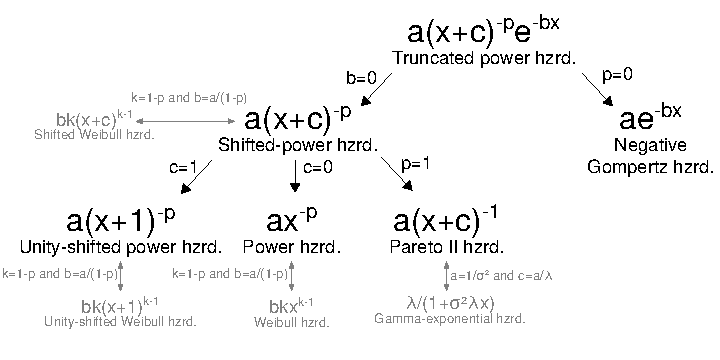
\includegraphics{fig/figure1.pdf}
\caption{\label{fig:plot-models}The exponentially-truncated shifted-power
family of hazards considered for the age-trajectory of infant mortality.
The family contains the negative Gompertz, Pareto II, and Weibull
hazards.}
\end{figure}

Prior to fitting the full truncated-hazard model to the data I will
discuss the respective properties and parameter interpretation of the
nested power- and negative Gompertz- hazards and demonstrate their fit
(or lack thereof) to the observed death rates of the complete cohort of
infants born in the US 2005 to 2009. This is to build evidence that it
takes both a power- and an exponential component to adequately describe
mortality over infancy, a subtlety that to my best knowledge has
remained unmentioned in the literature so far.

In a second analysis I test the fit of the truncated power hazard by
birth cohort, sex, APGAR score, gestation at birth, origin- and
education of the mother. Confronting a mortality model with such a
heterogeneous collection of life-tables acts as a validity test and
allows for the quantification of heterogeneous mortality trajectories
via comparison of model coefficients across population strata.
Particular attention will be paid to non-proportional variations of the
hazard, and to the behavior of the hazard during the neonatal period
(the first month of life) and during the post-neonatal period (months 1
to 12 of age).

All the models in this paper are fitted as generalized linear models
(GLMs). Such an approach guarantees concave likelihood surfaces and
consequently stable estimation of the model parameters while also
capitalizing on the wide availability of software to fit and evaluate
GLMs. By using suitable link functions and/or transformations of the age
variable a range of parametric hazard functions can be linearized and
thus fitted to observed age specific death counts and exposures via a
Poisson-GLM \citep{Aitkin1980, Clayton1983, Currie2016}.

The truncated power family of hazards (and therefore the nested negative
Gompertz, Weibull and Pareto hazards, see Figure \ref{fig:plot-models})
may be fit, after deciding on the value for \(c\), as Poisson-GLMs with
a log-link. This is possible due to the semi-linearity of
\(\mu_\text{TP}(x)\) on the log-scale:

\[
\log \mu_\text{TP}(x) = \log(a)-p\log(x+c)-bx = \beta_0+\beta_1\log(x+c)+\beta_2x,
\]

with \(a = \exp(\beta_0)\), \(p=-\beta_1\) and \(b=-\beta_2\). The
non-linear \(c\) parameter is estimated by maximizing the \emph{profile
likelihood} \citep{Murphy2000} of \(c\) over a range of GLM
fits.\footnote{Let \(\mathcal{L}(\boldsymbol\beta,c)\) be the full
  likelihood of a GLM fit with coefficients \(\boldsymbol\beta\) and
  age-offset \(c\). The profile likelihood of \(c\) is given by
  \(\mathcal{L}_{p}(c) = \max_{\boldsymbol\beta} \mathcal{L}(\boldsymbol\beta,c)\)
  and \(c\) is estimated as
  \(\hat c = \arg\max_{c}[\max_{\boldsymbol\beta} \mathcal{L}(\boldsymbol\beta,c)]\).
  I found \(\mathcal{L}_{p}(c)\) to be concave over \(c\) and the
  maximization was quick and stable.} Model inference is performed via
the model deviances, Pearson-residuals, and a pseudo-\(R^2\) criterion
based on the fitted models deviance versus the deviance of the null
(intercept-only) model. Confidence intervals around the parameter
estimates of the truncated power hazard are calculated from 1000
repeated fits of the model on 1000 different parametric-bootstrap
replicates of each life-table. Unlike the asymptotic standard errors
retrieved from the GLM fit the bootstrap approach incorporates the
uncertainty associated with the estimation of the non-linear \(c\)
parameter.

\section{The age-trajectory of US infant
mortality}\label{the-age-trajectory-of-us-infant-mortality}

The age-trajectory of infant mortality as observed in the US birth
cohort 2005-2009 is characterized by a peak at birth with a rapid
decline thereafter (see Figure \ref{fig:plot-imort}). While the
mortality rate over the first hour following birth is around 0.02
(deaths per person-day of exposure), 24 hours later the hazard is at
only \(1.1\,\%\) of its initial value and then again drops by a factor
of 10 over the next 29 days. Around one month after birth the hazard
starts to decline with a near constant relative-rate, approaching an
exponential behavior.

\begin{figure}
\centering
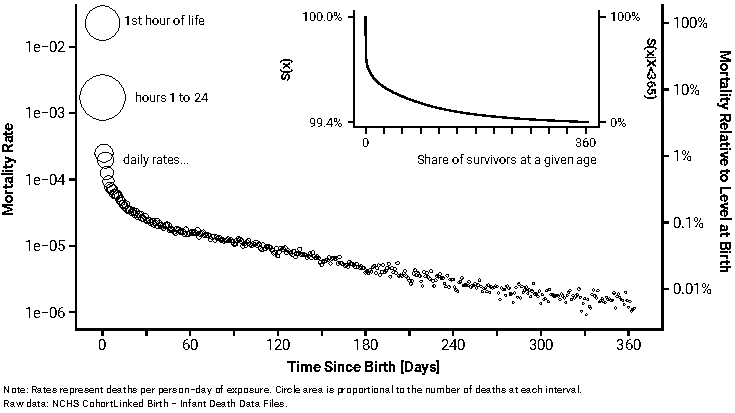
\includegraphics{fig/figure2.pdf}
\caption{\label{fig:plot-imort}Mortality rates over the first year of life
for the US birth cohort 2005-2009. Mortality drops rapidly during the
neonatal period after which it approches an exponential decline.}
\end{figure}

The pattern of a ``super-exponential'' decline in mortality during the
neonatal period followed by an exponential tail over the remainder of
the first year of life holds true for girls and boys, irrespective of
the social background of their mothers, the APGAR score upon birth, the
gestation at birth or birth cohort (see Figures \ref{fig:plot-apgar},
\ref{fig:plot-origin}, \ref{fig:plot-prematurity},
\ref{fig:plot-education}).

\section{Evidence for an exponentially-truncated power
hazard}\label{evidence-for-an-exponentially-truncated-power-hazard}

\begin{figure}
\centering
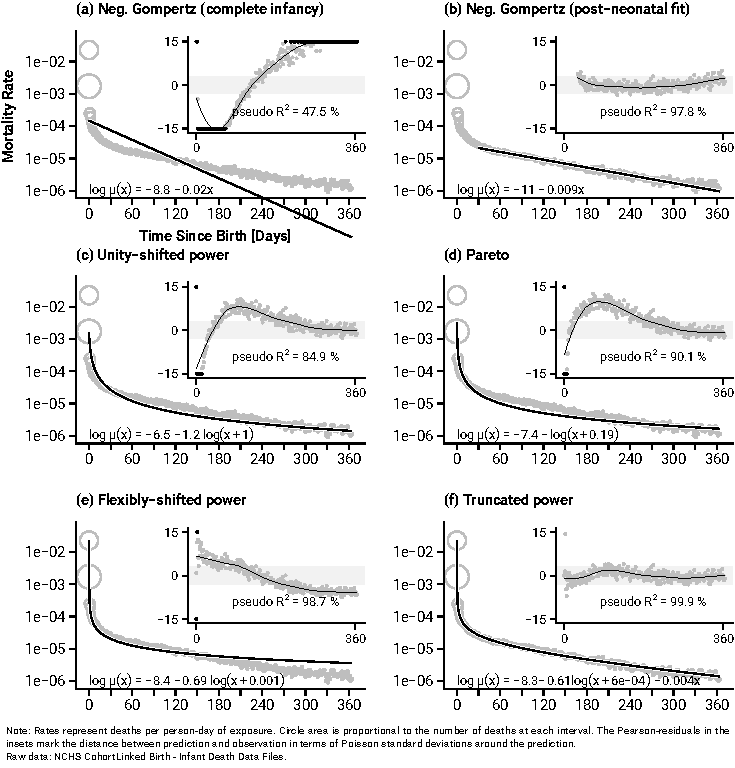
\includegraphics{fig/figure3.pdf}
\caption{\label{fig:plot-evidence}Fitted versus observed mortality over the
first year of life for the US birth cohort 2005-2009. Combining a
power-law and a negative Gompertz hazard in the truncated power model
(f) accounts for the different behavior of the hazard in the neonatal-
and post-neonatal periods and achieves a close fit over the entire first
year of life.}
\end{figure}

\subsection{Negative Gompertz hazard}\label{negative-gompertz-hazard}

\citet{Thiele1871}, in an early attempt to model mortality across the
whole human age-span, proposed to express the risk of death prior to
maturity as an exponential function of age,

\[
\mu_\text{GP}(x) = ae^{-bx},
\]

with \((x,a,b)\geq 0\). This is the hazard function of a Gompertz
distribution with a negative \(b\) parameter and therefore mirrors the
shape of the hazard commonly assumed for adult humans. The simplicity of
an exponential term for the hazard facilitates analytic treatment and
gives the parameters a direct interpretation as important quantities in
the study of infant mortality, \(\mu_\text{GP}(0)=a\) being the hazard
of death at the moment of birth and
\(-\frac{\mu'_\text{GP}(x)}{\mu_\text{GP}(x)}=b\) the instantaneous
relative rate of mortality decline over age. The fact that the risk
drops with a constant relative rate over age is the defining feature of
the negative Gompertz hazard. Related quantities are independent of age
as well: the time \(t\) it takes for the hazard to drop by a factor
\(k\) is the solution to equation
\(\frac{\mu_\text{GP}(x+t)}{\mu_\text{GP}(x)} = \frac{1}{k}\) given by
\(t_{1/k}=\frac{\log(k)}{b}\) and for each unit increase in age the
hazard changes by a factor
\(\frac{\mu_\text{GP}(x+1)}{\mu_\text{GP}(x)}=\exp(-b)\).

The negative Gompertz hazard can be expressed as a log-linear model with
Poisson distributed age-specific death counts \(D_x\) as outcome and
age-specific exposure times \(E_x\) as a fixed offset\footnote{Assuming
  that the width of each age group is small enough as to not introduce
  substantial aggregation bias.}

\[
\log\text{E}[D|x] = \beta_0 + \beta_1x + \log E_x, \text{with}~D\sim\text{Poisson}.
\]

From this fit the parameters of \(\mu_\text{GP}\) are recovered as
\(a = \exp(\beta_0)\) and \(b = -\beta_1\).

The negative Gompertz model of infant mortality is especially popular in
biology due to the influential paper by \citet{Siler1979} who included
it as part of his ``Competing-Risk Model for Animal Mortality''. In this
model a Gompertz term with negative \(b\) parameter is used ``to account
for the hazard due to immaturity'' \citep{Siler1979}. For life-tables of
human infants and children however, the negative Gompertz law has long
been found to provide an insufficient fit
\citetext{\citealp[p.~326]{Thiele1871}; \citealp{Choe1981}; \citealp{Gage1986}}.

\begin{table}[t]

\caption{\label{tab:tab-postneonatal}Number of months over the five year period 2005-2009 a negative Gompertz fit achieved a lower deviance on the post-neonatal cohort life-tables compared to a given power-law fit.}
\centering
\begin{tabular}{lll}
\toprule
\textbf{Gompertz vs.} & \textbf{Female} & \textbf{Male}\\
\midrule
Pareto II & 44/60 73.3\% & 54/60   90\%\\
Unity-shifted power & 59/60 98.3\% & 60/60  100\%\\
Flexibly-shifted power & 23/60 38.3\% & 41/60 68.3\%\\
\bottomrule
\multicolumn{3}{l}{\textsuperscript{} Raw data: US infants born in years 2005-2009. NCHS Cohort Linked}\\
\multicolumn{3}{l}{Birth - Infant Death Data Files.}\\
\end{tabular}
\end{table}

Figure \ref{fig:plot-evidence}a clearly shows that the age-trajectory of
infant mortality for the 2005-2009 US birth cohort deviates from a pure
log-linear (i.e.~exponential) form, ruling out the Gompertz hazard as a
suitable model for the entire infant age range. \emph{Yet}, a log-linear
decline constitutes a near perfect description of the mortality
trajectory over the post-neonatal period (Figure
\ref{fig:plot-evidence}b). The rate of death at day 30 after birth is
around 2.03 deaths per 100,000 person-days of exposure with a subsequent
decline of about \(0.93\,\%\) per additional day of age. Remarkably
these two numbers explain \(97.8\,\%\) of the total deviance in the data
during the post-neonatal period. Further investigating this result I fit
negative Gompertz and power-law hazards to the post-neonatal life-tables
for each of the 60 monthly US birth-cohorts from January 2005 to
December 2009 separate by sex. In the majority of the cases the negative
Gompertz hazard provided a closer fit to the observed post-neonatal
mortality trajectory than either of the alternative two or three
parameter power-law hazards (table \ref{tab:tab-postneonatal}).

\subsection{Power-law hazard}\label{power-law-hazard}

Various power laws have been specified to characterize the age-specific
hazard of infant death
\citep{Oppermann1870, Brillinger1961, Choe1981, DeBeer2016, Berrut2016}
all of which are variations on the basic expression

\[
\mu_\text{PW}(x)=ax^{-p},
\]

with \((a,p)\geq0\) and \(x>0\). Just like a negative Gompertz hazard, a
power-law hazard monotonically approaches 0 as \(x\rightarrow\infty\),
however, the relative rate of decline of a power hazard varies with age
according to
\(-\frac{\mu'_\text{PW}(x)}{\mu_\text{PW}(x)} =\frac{p}{x}\), i.e.~it is
greatest right after birth and approaches 0 as age increases. It is this
behavior that allows a power-law to initially decline faster than a
Gompertz hazard, yet become slower for larger \(x\), rendering it
potentially useful for the description of the day-to-day age pattern of
infant mortality.

Similar to the Gompertz case, the parameters of the power hazard can be
interpreted in terms of mortality level and rate-of-change: The risk of
death at age \(x=1\) is given by \(\mu_\text{PW}(1)=a\) and the
proportional change in mortality for change in age by proportion \(w\)
is \(\frac{\mu_\text{PW}(wx)}{\mu_\text{PW}(x)}=w^{-p}\). The
proportional increase in age \(w\) needed for the hazard to drop by
factor \(k\) is the solution to equation
\(\frac{\mu_\text{PW}(wx)}{\mu_\text{PW}(x)}=1/k\) given by
\(t_{1/k}= k^{\frac{1}{p}}\). The power parameter \(p\) by itself
represents the elasticity of the hazard,
\(\frac{\text{d}\log\mu_\text{PW}(x)}{\text{d}\log x}=-p\), i.e.~for
every infinitesimal proportional increase in age the hazard drops by
proportion \(p\). A convenient property of power laws is that the
elasticity is invariant to any re-scaling of age in the form \(x'=wx\).
In practice this means that the units used for the age column of the
infant life-tables (e.g.~hours, days, weeks) have no effect on the
estimation of the exponent \(p\).

Note that \(\mu_\text{PW}\) can be re-parametrized into the hazard of
the Weibull distribution \(\mu_\text{UW}(x)=bkx^{k-1}\) by substituting
\(p=1-k\) and \(a=bk\).

\citet{Berrut2016} fit \(\mu_\text{PW}\) to death rates starting shortly
after birth for a range of human and non-human populations and identify
power-law behavior in most populations.\footnote{Note that while
  occurrence-exposure rates are used in this article, \citet{Berrut2016}
  use the total number of births in the denominator of their
  death-rates.} Specifically they identify a segmented power-law
relationship between age and death rate for a cohort of Swiss infants.
The first segment starts 1 hour after birth and lasts for 8 hours, while
a different power coefficient is identified for the remainder of the
first month of life.

\subsubsection*{Unity-shifted power
hazard}\label{unity-shifted-power-hazard}
\addcontentsline{toc}{subsubsection}{Unity-shifted power hazard}

As \(x\) approaches 0, hazard \(\mu_\text{PW}\) approaches infinity. Due
to this behavior, a pure power-law hazard can not be used to describe
the age pattern of infant mortality starting from the moment of birth.
Instead one can either choose to exclude the moment/hour/day of birth
from the study period \citep[as did][]{Choe1981, Berrut2016} or add a
positive location parameter to \(\mu_\text{PW}\), i.e.
\(\mu_\text{PW}(x+c)\). The location parameter can either be estimated
from the data -- allowing for additional model flexibility -- or set to
some constant. The latter option has the advantage that the resulting
hazard can be written as a fully linear function of log-mortality. For
mathematical convenience one may use a unity offset resulting in the
\emph{unity-shifted power} expression

\[
\mu_\text{UP}(x) = a(x+1)^{-p},
\]

with \((x, a, p)\geq 0\). Due to the unity offset the risk of death at
the moment of birth is \(\mu_\text{UP}(0)=a\). The elasticity of
\(\mu_\text{UP}(x)\) approaches \(-p\) as \(x\rightarrow \infty\). In
practice I found \(-p\) to be a very close approximation to the true
elasticity of \(\mu_\text{UP}(x)\) for at least the post-neonatal
period, thus one may safely interpret \(p\) as the approximate
proportional drop in the hazard of infant death for an infinitesimal
proportional change in age starting at day 30 after birth.

The unity-shifted power hazard can be fitted as the log-linear Poisson
regression

\[
\log\text{E}[D|x] =
\beta_0 + \beta_1\log (x+1) + \log E_x,
\text{with}~D\sim\text{Poisson},
\]

with \(a = \exp(\beta_0)\) and \(p = -\beta_1\).

Note that \(\mu_\text{UP}\) can be translated into the unity-shifted
Weibull hazard \(\mu_\text{UW}(x)=bk(x+1)^{k-1}\) by substituting
\(k=1-p\) and \(b=a/(1-p)\).

While the unity-shifted power-law fits the 2005-2009 US infant
life-table better than the Gompertz hazard, the Pearson residuals in
Figure \ref{fig:plot-evidence}c still indicate a systematic
misspecification. Due to its very nature the unity-shifted power-law can
not capture the exponential portion of the hazard and it also fails to
adequately describe the extremely fast drop in the risk of death over
the first hours following birth.

\subsubsection*{Pareto hazard}\label{pareto-hazard}
\addcontentsline{toc}{subsubsection}{Pareto hazard}

In their model for the age pattern of human mortality \citet{DeBeer2016}
express the hazard of death during infancy and childhood as
\(\mu(x)=\frac{a}{c+x}\). This is the hazard function of a Pareto type
II distribution \citep[pp.~400]{Lomax1954, Marshall2007}. Rewriting the
hazard reveals a shifted power-law with exponent \(-1\), scaling factor
\(a\) and location offset \(c\),

\[
\mu_\text{PT}(x) = a(x+c)^{-1},
\]

where \((x, a)\geq 0\) and \(c > 0\). While for the unity-shifted
power-law the location offset is fixed and the power exponent varies,
the situation is reversed for the Pareto II hazard with a fixed power
and a variable location offset. As \(\mu_\text{PT}(x)\) is finite for
\(x>-c\) one may interpret the \(c\) parameter as the duration
\(\mu_\text{PT}\) extends into the pre-natal period. For such an
interpretation to be justified the intrapartum death-rates (death during
labor, i.e.~at \(x<0\)) have to follow the same functional form as the
infant death rates and, given that \(\mu(x+c)\) is declining with age,
have to be higher than the mortality rates after birth. Of course the
mortality at birth is \(\mu_\text{PT}(0)=a/c\) with \(a\) being the
hazard level at \(x=1-c\). The elasticity of the Pareto hazard is
\(\frac{\text{d}\log\mu_\text{PT}(x)}{\text{d}\log x}=-\frac{x}{x+c}\)
which approaches \(-1\) as \(x\rightarrow\infty\). This implies a
central characteristic of the Pareto hazard, namely that in the limit
any proportional increase in age by factor \(w\) results in a
proportional change of the hazard by \(1/w\), e.g.~doubling age halves
the hazard. In practice the estimated values for \(c\) are small enough
for this limiting behavior to set in shortly after birth.

The Pareto hazard can be fitted as

\[
\log\text{E}[D|x] = \beta_0 - \log(x+c) + \log E_x,~\text{with}~D\sim\text{Poisson},
\]

an intercept-only model with additional offset \(-\log(x+c)\) and
\(a=\exp(\beta_0)\). As described earlier \(c\) is estimated by
maximizing its profile-likelihood.

\citet{Vaupel1983} propose to describe the infant/childhood component of
human mortality by a Gamma-Exponential frailty model with population
hazard function \(\mu_\text{GE}(x)=\lambda/(1+\sigma^2\lambda x)\),
i.e.~a continuous mixture distribution of constant baseline hazards
(corresponding to an exponential baseline distribution of deaths) with
Gamma-distributed rate parameter \(\lambda\). As noted by
\citet{Wienke2011} this model is equivalent to \(\mu_\text{PT}\) when
\(a=1/\sigma^2\), i.e.~the inverse of the variance parameter of the
Gamma-Exponential frailty model, and \(c = a/\lambda\). Therefore
\(\mu_\text{PT}\) may be interpreted as the population hazard resulting
from mortality selection among individuals with constant hazards of
Gamma-varying magnitudes.

The fit of the Pareto hazard to the 2005-2009 US infant life-tables is
inadequate and similar to that of the shifted-power-law (Figure
\ref{fig:plot-evidence}d).

\subsubsection*{Flexibly-shifted power
hazard}\label{flexibly-shifted-power-hazard}
\addcontentsline{toc}{subsubsection}{Flexibly-shifted power hazard}

Adding a positive location offset \(c\) to \(\mu_\text{PW}\) results in
the flexibly-shifted power hazard

\[
\mu_\text{FP}(x) = a(x+c)^{-p},
\]

where \((x,a,b)\geq 0\) and \(c > 0\). This hazard shape contains the
Pareto II hazard and the unity-shifted power hazard as special cases.
Note that \(\mu_\text{FP}\) can be interpreted as the hazard function of
the shifted Weibull distribution \(\mu_\text{SW}(x)=bk(x+c)^{k-1}\) with
\(k=1-p\) and \(b=a/(1-p)\).

The elasticity of the flexibly-shifted power hazard is
\(\frac{\text{d}\log\mu_\text{FP}(x)}{\text{d}\log x}=-\frac{px}{x+c}\)
which approaches \(-p\) as \(x\rightarrow\infty\). Due to small
estimates for \(c\) this limiting behavior sets in shortly after birth,
allowing an interpretation of the \(p\) parameter as the proportional
drop in mortality for an infinitesimal proportional increase in age for
all but the very first moments after birth. As for the Pareto II hazard
parameter \(a\) is the hazard level at age \(1-c\) and \(c\) may be
interpreted as the time that \(\mu_\text{FP}\) extends into the
pre-natal period.

The flexibly-shifted power hazard can be fitted as a Poisson-GLM of the
form

\[
\log\text{E}[D|x] = \beta_0 + \beta_1\log(x+c) + \log E_x,~\text{with}~D\sim\text{Poisson},
\]

with the original parameters recovered as \(a = \exp(\beta_0)\) and
\(p = -\beta_1\). Just as for the Pareto hazard \(c\) is estimated by
maximizing its profile-likelihood.

Allowing for both a free power parameter \(p\) and a free location
offset \(c\) greatly improves the fit to the US 2005-2009 infant
life-tables compared to the more restricted unity-shifted power and
Pareto hazards (Figure \ref{fig:plot-evidence}e). The estimate for \(c\)
is 0.0012 (i.e.~a location shift by \(\approx1.7\) minutes of age) and
for \(p\) equals 0.69, corresponding to an approximate drop in mortality
by \((1-2^{-0.69})\times100=38 \%\) for every doubling of age. While
fitting better than the hazards discussed above, the Pearson residuals
in Figure \ref{fig:plot-evidence}e still exhibit a clear curvature
signifying a systematic lack of fit.

\subsection{Exponentially-truncated power-law
hazard}\label{exponentially-truncated-power-law-hazard}

Multiplying the flexibly-shifted power-law hazard \(\mu_\text{FP}\) with
an exponential term results in the exponentially-truncated power
expression

\[
\mu_\text{TP}(x) = a(x+c)^{-p}e^{-bx},
\]

with \((x, a, p, b)\geq 0\) and \(c>0\). This hazard contains all of the
above models as special cases (see Figure \ref{fig:plot-models}).

The power-component of the hazard is said to be ``truncated'' by the
exponential component because with increasing age \(\mu_\text{TP}\)
approaches a constant relative rate of change, formally
\(\lim_{x\to\infty}\frac{\mu'_\text{TP}(x)}{\mu_\text{TP}(x)}=-b\).

The Poisson-GLM form of the truncated power hazard is

\[
\log\text{E}[D|x] = \beta_0 + \beta_1\log(x+c) + \beta_2x+\log E_x,~\text{with}~D\sim\text{Poisson},
\]

where \(a = \exp(\beta_0)\), \(p = -\beta_1\), \(b = -\beta_2\) and the
non-linear coefficient \(c\) is estimated via profile-likelihood
maximization.

Adding the exponential term to \(\mu_\text{FP}\) significantly
(\(p<0.001\) via deviance-ratio test) improves the fit of the
Poisson-GLM to the 2005-2009 US birth cohort and flattens the trend in
the Pearson residuals over age (Figure \ref{fig:plot-evidence}f). Infant
mortality over age eventually follows an exponential trajectory -- a
result that, as will be demonstrated, holds true for different
birth-cohorts, by sex, medical and social strata.

\section{Evaluation of the truncated power
hazard}\label{evaluation-of-the-truncated-power-hazard}

The exponentially truncated power-law hazard achieves an excellent fit
irrespective of cohort, sex, five minute APGAR score, gestational age at
birth, origin or education of the mother. In all life-tables under
consideration the percentage of deviance explained by the model ranges
from 94.5\% to 99.6\%. For every single population the inclusion of an
exponential term in addition to the shifted-power term significantly
(\(p<0.001\) via deviance-ratio tests) improves the fit, reducing the
residual deviance by more than 50\% on 43 out of the 56 populations
(Table \ref{tab:tab-deviances}).

\begin{table}[t]

\caption{\label{tab:tab-deviances}Percent reduction in residual deviance after truncating the power-law hazard with an exponential term. All results significant at $p<0.001$ (via deviance ratio tests).}
\centering
\begin{tabular}{llcccc}
\toprule
\multicolumn{2}{c}{\textbf{ }} & \multicolumn{2}{c}{\textbf{1995-1999}} & \multicolumn{2}{c}{\textbf{2005-2009}} \\
\cmidrule(l{3pt}r{3pt}){3-4} \cmidrule(l{3pt}r{3pt}){5-6}
\textbf{} & \textbf{} & \textbf{Female} & \textbf{Male} & \textbf{Female} & \textbf{Male}\\
\midrule
 & Very low [0,5) & 50.2 & 45.6 & 61.3 & 60.3\\

 & Low [5,9) & 20.6 & 27.9 & 49.5 & 49.7\\

\multirow{-3}{*}{\raggedright\arraybackslash APGAR} & Regular 9+ & 86.8 & 86.4 & 89.8 & 92.0\\
\cmidrule{1-6}
 & Non-Hispanic Black & 56.0 & 60.1 & 65.1 & 63.9\\

 & Non-Hispanic White & 76.3 & 74.2 & 81.9 & 79.6\\

 & Hispanic & 55.4 & 63.6 & 60.2 & 69.4\\

\multirow{-4}{*}{\raggedright\arraybackslash Origin} & Other & 20.3 & 29.4 & 24.7 & 33.5\\
\cmidrule{1-6}
 & Extremely preterm <28w & 67.4 & 67.1 & 74.1 & 75.7\\

 & Very preterm [28,32)w & 54.7 & 56.1 & 60.9 & 63.0\\

 & Moderate to late preterm [32,37)w & 58.2 & 60.0 & 71.0 & 70.2\\

\multirow{-4}{*}{\raggedright\arraybackslash Prematurity} & Term 37w+ & 79.8 & 78.1 & 83.7 & 80.9\\
\cmidrule{1-6}
 & Elementary or less & 38.6 & 41.9 & 30.5 & 40.9\\

 & High school & 76.9 & 74.7 & 79.9 & 77.3\\

\multirow{-3}{*}{\raggedright\arraybackslash Education} & College or university & 67.3 & 66.0 & 76.6 & 76.8\\
\bottomrule
\multicolumn{6}{l}{\textsuperscript{} Raw data: US infants born in years 2005-2009. NCHS Cohort Linked Birth - Infant Death Data Files.}\\
\end{tabular}
\end{table}

The shape of the hazard function over age varies most strongly by APGAR
score (Figure \ref{fig:plot-apgar}). The exponential behavior of the
hazard is most pronounced for the population of infants born with a
score of 9 or 10 (the majority of infants born). Within two weeks after
delivery the initial mortality spike at birth transitions into a
log-linear decline in mortality-risk of around 0.7\% per day.
Conversely, the hazard trajectory of the life-table for infants with a
``low'' APGAR score (indicating health problems of upon delivery), while
still exponential in the tail, features a more gradual transition into
log-linear behavior. The greatest difference in the behavior of the
hazard among the APGAR groups can be seen over the first week of life.
While for APGAR group 0 to 5 the hazard drops by a factor of 1000 from
the day of birth to an age of seven days it only drops by a factor of 9
or less for the other groups. Thus hazards vary by APGAR score in a
highly \emph{non-proportional} fashion as can also be inferred from the
varying power (\(p\)), exponential-rate (\(b\)) and offset (\(c\))
parameters of the fitted models. Non-proportional behavior, albeit less
pronounced, is also evident when comparing hazards by prematurity, with
higher values for the power parameter \(p=-\beta_1\) for lower ages of
gestation at birth\footnote{A result also observed by \citet{Berrut2016}
  for Swiss and Norwegian infants after fitting a simple power-law to
  age specific mortality rates.} (Figure \ref{fig:plot-prematurity}).

The relative rate of mortality decline during the post-neonatal period
(as approximated by \(b\)) is higher for premature infants and infants
with a low APGAR score compared to infants born at term or with a
regular APGAR score. This implies that the relative difference in
mortality between very frail and less frail infants diminishes over age
to some degree.

Hazards are mostly proportional by ethnicity of the mother (Figure
\ref{fig:plot-origin}) with the risk of death during the later stages of
infancy declining exponentially with a rate of \(0.3\) to \(0.5\%\) per
day of age and the power parameter ranging from \(-0.51\) to \(-0.55\)
across the life-table strata. Notably during the post-neonatal period
mortality over age declines slower for children of African-American
mothers compared to infants of white mothers\footnote{Significant at
  \(p<0.05\) for female and male infants of either birth cohort, see
  table \ref{tab:tab-ci-b} in the appendix and associated
  non-overlapping 95\% confidence intervals around the \(b\) parameter
  for African-American and white mothers.}; taken together with the
observation that the intercept of the hazard curve is highest among
infants of African-American mothers, this puts the group at a double
disadvantage. Along education strata the hazards are proportional
(Figure \ref{fig:plot-education}).

Apart from a proportionally higher hazard for males compared to females
there are no systematic differences in the age-trajectory of infant
mortality between the sexes. Similarly the difference between the two
birth cohorts is mostly proportional with the younger cohort having a
lower intercept \(\beta_0\) (Figures
\ref{fig:plot-apgar}--\ref{fig:plot-education}).

\begin{figure}
\centering
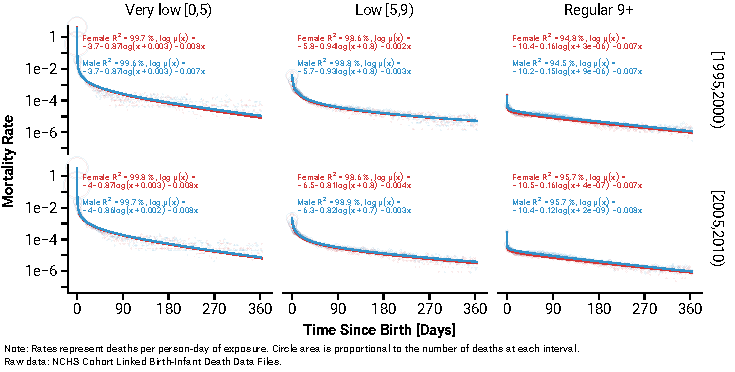
\includegraphics{fig/figure4.pdf}
\caption{\label{fig:plot-apgar}Age specific hazard of death as predicted by
the truncated power model contrasted with observed daily mortality rates
by sex, birth-cohort, and 5-minute APGAR score.}
\end{figure}

\begin{figure}
\centering
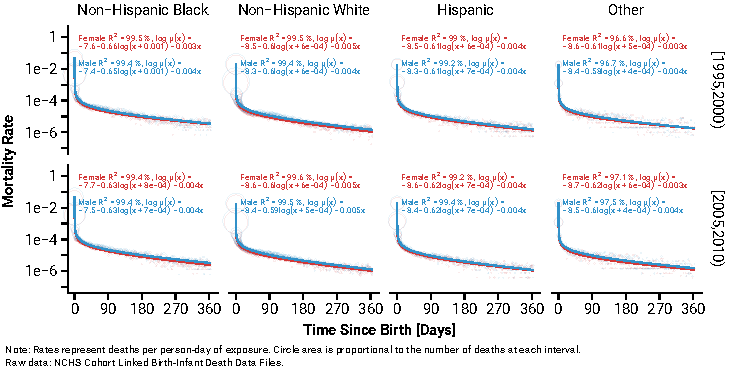
\includegraphics{fig/figure5.pdf}
\caption{\label{fig:plot-origin}Age specific hazard of death as predicted by
the truncated power model contrasted with observed daily mortality rates
by sex, birth-cohort, and ethnicity of the mother.}
\end{figure}

\begin{figure}
\centering
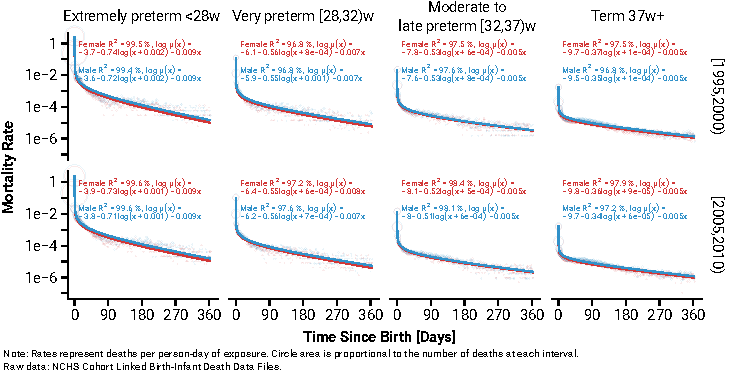
\includegraphics{fig/figure6.pdf}
\caption{\label{fig:plot-prematurity}Age specific hazard of death as
predicted by the truncated power model contrasted with observed daily
mortality rates by sex, birth-cohort, and prematuriy.}
\end{figure}

\begin{figure}
\centering
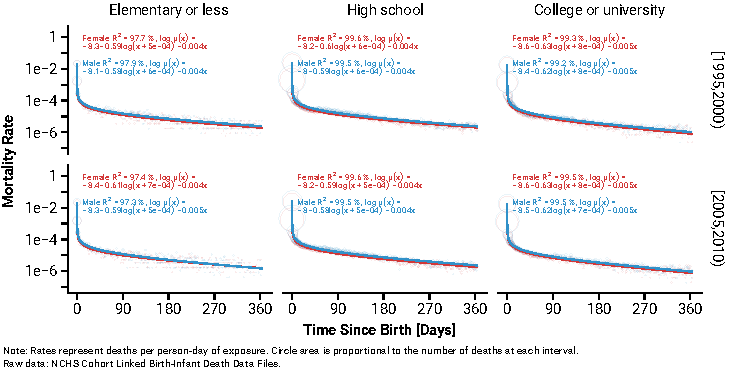
\includegraphics{fig/figure7.pdf}
\caption{\label{fig:plot-education}Age specific hazard of death as predicted
by the truncated power model contrasted with observed daily mortality
rates by sex, birth-cohort, and education of mother.}
\end{figure}

\section{Interpretation of the truncated power
hazard}\label{interpretation-of-the-truncated-power-hazard}

\subsection{A shock-recovery process}\label{a-shock-recovery-process}

The power-exponential product of the population hazard \(\mu_\text{TP}\)
can be interpreted as a \emph{non-homogeneous split Poisson process},
where \emph{shocks} to an infants health arrive with rate \(\lambda(x)\)
per unit person-time, each shock resulting in infant death with
probability \(p(x)\).\footnote{Shock models in the context of human
  mortality have for example been studied by \citet{Strehler1960},
  \citet{Finkelstein2005}, \citet{Cha2016}.}

Let \(N(x)\) be the number of infants alive at age \(x\) and let
\(\text{E}{[M]}\) be the expected value of a Poisson distributed random
variable \(M\) with rate parameter \(\int_x^{x+n}\lambda(x)N(x)\)
representing the total number of \emph{health-shocks} the population of
infants is expected to experience over age interval \([x, x+n)\). If
each shock leads to death with probability \(p(x)\) then the number of
deaths \(D\) over age interval \([x, x+n)\) follows a Poisson
distribution with expected value

\[
\text{E}[{}_{n}D_x]=\int_x^{x+n}\lambda(x)p(x)N(x)\,\text{d}x,
\]

see \citet{Prekopa1958} for a proof. The hazard of death experienced by
survivors \(N\) at time \(x\) is \(\mu(x) = \lambda(x)p(x)\). If the
rate of shocks \(\lambda(x)\) varies over time according to a
flexibly-shifted power hazard and if the probability of a shock leading
to death \(p(x)\) is exponentially declining the truncated power-law
hazard is recovered. Note that neither the rate of shocks nor the
probability of death following a shock are identified as this would
require inferring the model \(\mu(x)=a_1(x+c)^{-p}\times a_2e^{-bx}\)
from the fit \(\mu(x)=a(x+c)^{-p}e^{-bx}\) -- a problem with infinitely
many solutions. However, the power and the exponential rate parameters
\(p\) and \(b\) are completely identified and can be interpreted as
follows: For the extremely preterm female births of the US birth cohort
1995-1999 (Figure \ref{fig:plot-evidence}f) the rate of shocks,
\(\lambda(x)\propto(x+0.002)^{-0.74}\), declined rapidly in the vicinity
of birth by approximately \((1-2^{-0.74})\times100=40\,\%\) for every
doubling of age whereas the probability of a shock leading to death,
\(p(x)\propto e^{-bx}\), declined by about \(0.9\,\%\) per additional
day of age.

Why should we use the power-law for the rate of shocks and the
exponential term for the probability of a shock leading to death instead
of the other way around -- after all both options lead to the same
expression for \(\mu(x)\)? I find it likely that the rapid neonatal
mortality decline is predominantly a result of the waning stresses of
birth -- a sudden transition which may inflict a series of ``shocks'' to
the infant -- and not the result of a fast decline in the mortality risk
associated with each shock. Furthermore, as
\(\lim_{x\to\infty}\frac{\mu'_\text{FP}(x)}{\mu_\text{FP}(x)}=0\), the
power-law approaches a constant hazard as age increases, allowing it to
capture the age-independent rate of accidents which may dominate the
rate of shocks later in infancy.

A very specific shock-recovery process is described by the
Strehler-Mildvan model of senescent mortality. \citet{Strehler1960}
propose a model where individuals experience shocks to their health at a
constant rate \(\alpha\). The magnitude of each shock, ranging from mild
to severe, is a value drawn from an exponential random variable with
rate \(\beta\). The shocks are counteracted by the vitality of an
individual which is a positive and declining function of age. When the
magnitude of a shock at age \(x\) exceeds the individual's vitality at
that age, death occurs. \citet{Strehler1960} show that this process
leads to a Gompertz distribution of life-times with corresponding hazard
function \(\mu(x)=\alpha e^{\beta x}\).

The truncated power hazard of infant mortality can be derived from such
a Strehler-Mildvan process by changing two assumptions: 1) Where
\citet{Strehler1960} assume a decrease of vitality with time due to
ageing one assumes an increase due to growth, and 2) instead of that
shocks arrive with a constant rate \(\alpha\) one assumes that the risk
of experiencing complications is highest at birth and falls over time
(according to a shifted Weibull distribution).

\subsection{A mortality selection
process}\label{a-mortality-selection-process}

In the multiplicative frailty model \citep{Vaupel1979} it is assumed
that all individuals in a population share the same age specific
``baseline hazard'' of death \(\mu_0(x)\) but on different ``frailty''
levels \(z\) which act multiplicatively on the baseline. Consequently
the age specific hazard conditioned on frailty is given by

\[
\mu(x|z) = z\mu_0(x).
\]

Frailty is treated as a random variable \(Z\) with density \(f(z|x)\) at
age \(x\). Integrating out the frailty yields the expression for the
hazard observed at the population level, which is a mixture of the
individual level hazards weighted by the age specific distribution of
frailties

\[
\overline{\mu}(x) = \int_0^\infty \mu(x|z)f(z|x)\,\text{d}z,
\]

which may be re-expressed as

\[
\overline{\mu}(x) = \mu_0(x)\int_0^\infty zf(z|x)\,\text{d}z = \mu_0(x)\text{E}[Z|x],
\]

showing that the population hazard is a product of the baseline hazard
and the average frailty among the population at age \(x\). By choosing
\(\mu_0(x)=ae^{-bx}\) and \(\text{E}[Z|x]=(x+c)^{-p}\) we express the
truncated power-law hazard \(\mu_\text{TP}\) as a multiplicative frailty
model.

Frailty models can be interpreted in terms of \emph{mortality
selection}: Because individuals with a high frailty on average die
earlier than those with lower values for \(z\) the average frailty among
a cohort of individuals declines over time. Above we modeled this
decline as a shifted power function of age and consequently \(p\) can be
interpreted as the approximate elasticity of average frailty w.r.t. age,
0.69 for the US birth cohort 2005-1999, corresponding to an approximate
drop in average frailty by \(38\,\%\) for every doubling of age -- a
substantial mortality selection shortly after birth.

While differing in frailty, all individuals of a cohort are assumed to
share the same baseline hazard. By modelling this \emph{individual
level} risk as an exponential function of age we assume that each
additional unit of age decreases an infants risk of death by factor
\(\exp(-b)\), around \(0.4\,\%\) per additional day of age for the
2005-1999 US birth cohort (Figure \ref{fig:plot-evidence}f). This
relatively slow rate of decline may be attributed to \emph{acquired
robustness} due to the infants continued growth and development.

Of course one could, to the same effect, also choose
\(\mu_0(x)=a(x+c)^{-p}\) and \(\text{E}[Z|x]=e^{-bx}\). This model
implies that the power-law behavior of the population hazard (mostly
seen during the first month of life) arises from individual level
processes, while above we have assumed that the rapid mortality decline
after birth is mostly due to changing average frailty, i.e.~mortality
selection. Different choices for the baseline hazard and the
distribution of frailties can result in the same expression for the
population hazard -- an identifiability problem which is well known in
the frailty-model literature \citep[e.g.][]{Hougaard1995}.

\section{Discussion}\label{discussion}

Using highly detailed individual level data on the timing of death over
the first year of life I found strong evidence for an exponentially
truncated power-law behavior of the hazard of infant death in two recent
US birth cohorts. The shift from a power-law regime to an exponential
decline has not been noted in the literature before and invites
speculation regarding the mechanisms that give rise to such a pattern.
Observed hazards may be the result of mechanisms which have been
discussed at length in the context of senescent risk of death: mortality
selection due to heterogeneous frailties and a shock-recovery process.

The frailty hypothesis may be tested via a decomposition analysis.
\citet{Vaupel2010a} prove that, if the population hazard
\(\overline\mu(x)\) and the stratum specific hazards \(\mu(x|z)\) are
known for a cohort, then the rate of change over age of
\(\overline\mu(x)\) can be decomposed into a ``direct change'' component
and change due to the process of mortality selection. Using this
decomposition one could for example calculate how much of the decline in
the risk of death over the first week of life as shown in Figure
\ref{fig:plot-imort} is due the changing population composition by
prematurity status resulting from the early death of extremely premature
infants, i.e.~mortality selection.

A test of the shock-recovery model is less straightforward as it
requires both a clear definition of what constitutes a shock and data on
the timing of such shocks to see if their rate of occurrence corresponds
to either the exponential or the power-law component of the truncated
power-law hazard.

Note that the truncated power hazard discussed in this paper does not
permit an interpretation as a competing-risks model. Such a model was
implied by \citet{Bourgeois-Pichat1951} for the age-trajectory of infant
mortality, which he partitioned into deaths due to congenital disorders
and deaths due to accidents. An alternative competing-risks model
featuring a power-law and an exponential term could take the form
\(\mu_\text{CR}(x)=a_1(x+c)^{-p} + a_2\exp(-bx)\), which may be
re-written as
\(\mu_\text{CR}(x)=\exp[\log a_1 - p\log(x+c)] + \exp[\log a_2 - bx]\).
Sums-of-exponentials can be fit in the GLM framework by using a
composite-link-function \citep{Thompson1981, Camarda2016}. Assuming that
deaths due to intrinsic causes follow a power-law behavior whereas
extrinsic deaths feature the hazard of a negative-Gompertz distribution,
this competing-risks formulation of the age-specific hazard of infant
death over time permits a shape-based cause-of-death decomposition.

The results of this paper indicate that the proportional hazards
assumption does not hold across APGAR score and prematurity strata. The
association of those variables with the baseline hazard of death over
the first year of life is highly non-proportional with much of the
``effect'' focused on the first weeks of life. Indeed differences in the
rate of post-neonatal mortality decline imply that the relative
difference in mortality between very frail and less frail infants
diminishes over age to some degree.

Insofar as the truncated power hazard generalizes to populations other
than present day US it can become a valuable tool for working with
low-quality data on the timing of infant deaths. Based on
\(\mu_\text{TP}\) one can calculate life-table \(a_0\) from coarse data;
design model infant-life-tables; smooth over data artifacts such as
age-heaping; estimate seasonal effects on mortality separately from age
effects; or include realistic infant mortality schedules into a
simulation model.

\clearpage

\section*{Appendix: Parameter estimates and confidence intervals for the
truncated power
hazard}\label{appendix-parameter-estimates-and-confidence-intervals-for-the-truncated-power-hazard}
\addcontentsline{toc}{section}{Appendix: Parameter estimates and
confidence intervals for the truncated power hazard}

\begin{table}[t]

\caption{\label{tab:tab-ci-M}The factor of mortality reduction over the first 7 days of life. Parameter estimates and $95\%$ CIs calculated from the truncated-power hazard GLM fits for various US infant cohorts.}
\centering
\begin{tabular}{llll}
\toprule
\textbf{} & \textbf{} & \textbf{Female} & \textbf{Male}\\
\midrule
\addlinespace[0.3em]
\multicolumn{4}{l}{\textbf{1995-1999}}\\
 & Very low [0,5) & 1011 (826, 1242) & 962 (810, 1157)\\

 & Low [5,9) & 8 (6, 10) & 8 (6, 10)\\

\multirow{-3}{*}{\raggedright\arraybackslash \hspace{1em}APGAR} & Regular 9+ & 10 (7, 14) & 8 (5, 10)\\
\cmidrule{1-4}
 & Non-Hispanic Black & 328 (282, 385) & 315 (277, 357)\\

 & Non-Hispanic White & 303 (272, 340) & 275 (249, 304)\\

 & Hispanic & 320 (262, 391) & 277 (229, 331)\\

\multirow{-4}{*}{\raggedright\arraybackslash \hspace{1em}Origin} & Other & 329 (228, 498) & 303 (219, 444)\\
\cmidrule{1-4}
 & Extremely preterm <28w & 524 (449, 604) & 448 (399, 508)\\

 & Very preterm [28,32)w & 181 (135, 246) & 145 (113, 188)\\

 & Moderate to late preterm [32,37)w & 147 (116, 185) & 127 (103, 158)\\

\multirow{-4}{*}{\raggedright\arraybackslash \hspace{1em}Prematurity} & Term 37w+ & 58 (49, 67) & 49 (43, 57)\\
\cmidrule{1-4}
 & Elementary or less & 281 (203, 385) & 236 (178, 316)\\

 & High school & 280 (254, 312) & 256 (232, 281)\\

\multirow{-3}{*}{\raggedright\arraybackslash \hspace{1em}Education} & College or university & 330 (286, 377) & 303 (268, 345)\\
\cmidrule{1-4}
\addlinespace[0.3em]
\multicolumn{4}{l}{\textbf{2000-2005}}\\
 & Very low [0,5) & 1039 (866, 1241) & 1008 (869, 1193)\\

 & Low [5,9) & 6 (5, 8) & 7 (5, 8)\\

\multirow{-3}{*}{\raggedright\arraybackslash \hspace{1em}APGAR} & Regular 9+ & 14 (11, 18) & 13 (10, 16)\\
\cmidrule{1-4}
 & Non-Hispanic Black & 318 (272, 373) & 340 (299, 391)\\

 & Non-Hispanic White & 301 (268, 338) & 277 (250, 304)\\

 & Hispanic & 326 (278, 389) & 310 (268, 359)\\

\multirow{-4}{*}{\raggedright\arraybackslash \hspace{1em}Origin} & Other & 348 (243, 508) & 347 (258, 472)\\
\cmidrule{1-4}
 & Extremely preterm <28w & 538 (471, 613) & 477 (427, 531)\\

 & Very preterm [28,32)w & 194 (152, 249) & 178 (141, 225)\\

 & Moderate to late preterm [32,37)w & 142 (115, 175) & 119 (98, 144)\\

\multirow{-4}{*}{\raggedright\arraybackslash \hspace{1em}Prematurity} & Term 37w+ & 60 (51, 69) & 58 (50, 66)\\
\cmidrule{1-4}
 & Elementary or less & 310 (221, 436) & 290 (218, 397)\\

 & High school & 280 (248, 312) & 272 (248, 300)\\

\multirow{-3}{*}{\raggedright\arraybackslash \hspace{1em}Education} & College or university & 320 (285, 366) & 315 (282, 351)\\
\bottomrule
\multicolumn{4}{l}{\textsuperscript{} Raw data: US infants born in years 2005-2009. NCHS Cohort Linked Birth - Infant Death Data Files.}\\
\end{tabular}
\end{table}

\clearpage

\begin{table}[t]

\caption{\label{tab:tab-ci-a}Estimated $a$ parameters of truncated-power hazard GLM fits for various US infant cohorts. Mean estimates and $95\%$ confidence intervals are based on 1000 parametric bootstrap replications.}
\centering
\begin{tabular}{llll}
\toprule
\textbf{} & \textbf{} & \textbf{Female} & \textbf{Male}\\
\midrule
\addlinespace[0.3em]
\multicolumn{4}{l}{\textbf{1995-1999}}\\
 & Very low [0,5) & 2.5e-02 (2.5e-02, 2.6e-02) & 2.6e-02 (2.5e-02, 2.6e-02)\\

 & Low [5,9) & 2.9e-03 (2.7e-03, 3.2e-03) & 3.3e-03 (3.1e-03, 3.6e-03)\\

\multirow{-3}{*}{\raggedright\arraybackslash \hspace{1em}APGAR} & Regular 9+ & 3.0e-05 (2.9e-05, 3.2e-05) & 3.8e-05 (3.6e-05, 3.9e-05)\\
\cmidrule{1-4}
 & Non-Hispanic Black & 4.8e-04 (4.7e-04, 4.9e-04) & 5.8e-04 (5.7e-04, 5.9e-04)\\

 & Non-Hispanic White & 2.0e-04 (1.9e-04, 2.0e-04) & 2.5e-04 (2.4e-04, 2.5e-04)\\

 & Hispanic & 2.0e-04 (1.9e-04, 2.0e-04) & 2.4e-04 (2.3e-04, 2.4e-04)\\

\multirow{-4}{*}{\raggedright\arraybackslash \hspace{1em}Origin} & Other & 1.8e-04 (1.8e-04, 1.9e-04) & 2.1e-04 (2.1e-04, 2.2e-04)\\
\cmidrule{1-4}
 & Extremely preterm <28w & 2.4e-02 (2.3e-02, 2.4e-02) & 2.8e-02 (2.7e-02, 2.8e-02)\\

 & Very preterm [28,32)w & 2.2e-03 (2.1e-03, 2.3e-03) & 2.7e-03 (2.6e-03, 2.8e-03)\\

 & Moderate to late preterm [32,37)w & 4.3e-04 (4.1e-04, 4.4e-04) & 4.9e-04 (4.8e-04, 5.0e-04)\\

\multirow{-4}{*}{\raggedright\arraybackslash \hspace{1em}Prematurity} & Term 37w+ & 6.3e-05 (6.2e-05, 6.5e-05) & 7.5e-05 (7.3e-05, 7.6e-05)\\
\cmidrule{1-4}
 & Elementary or less & 2.5e-04 (2.4e-04, 2.6e-04) & 2.9e-04 (2.8e-04, 3.1e-04)\\

 & High school & 2.7e-04 (2.7e-04, 2.8e-04) & 3.4e-04 (3.4e-04, 3.4e-04)\\

\multirow{-3}{*}{\raggedright\arraybackslash \hspace{1em}Education} & College or university & 1.9e-04 (1.8e-04, 1.9e-04) & 2.2e-04 (2.2e-04, 2.3e-04)\\
\cmidrule{1-4}
\addlinespace[0.3em]
\multicolumn{4}{l}{\textbf{2000-2005}}\\
 & Very low [0,5) & 1.8e-02 (1.8e-02, 1.8e-02) & 1.8e-02 (1.7e-02, 1.8e-02)\\

 & Low [5,9) & 1.6e-03 (1.4e-03, 1.7e-03) & 1.8e-03 (1.7e-03, 2.0e-03)\\

\multirow{-3}{*}{\raggedright\arraybackslash \hspace{1em}APGAR} & Regular 9+ & 2.7e-05 (2.6e-05, 2.8e-05) & 3.1e-05 (3.0e-05, 3.2e-05)\\
\cmidrule{1-4}
 & Non-Hispanic Black & 4.5e-04 (4.4e-04, 4.6e-04) & 5.4e-04 (5.3e-04, 5.5e-04)\\

 & Non-Hispanic White & 1.9e-04 (1.8e-04, 1.9e-04) & 2.3e-04 (2.3e-04, 2.3e-04)\\

 & Hispanic & 1.8e-04 (1.8e-04, 1.9e-04) & 2.2e-04 (2.2e-04, 2.3e-04)\\

\multirow{-4}{*}{\raggedright\arraybackslash \hspace{1em}Origin} & Other & 1.7e-04 (1.6e-04, 1.8e-04) & 2.0e-04 (1.9e-04, 2.1e-04)\\
\cmidrule{1-4}
 & Extremely preterm <28w & 2.0e-02 (1.9e-02, 2.0e-02) & 2.3e-02 (2.3e-02, 2.3e-02)\\

 & Very preterm [28,32)w & 1.7e-03 (1.6e-03, 1.8e-03) & 2.0e-03 (1.9e-03, 2.1e-03)\\

 & Moderate to late preterm [32,37)w & 3.0e-04 (2.9e-04, 3.0e-04) & 3.2e-04 (3.2e-04, 3.3e-04)\\

\multirow{-4}{*}{\raggedright\arraybackslash \hspace{1em}Prematurity} & Term 37w+ & 5.3e-05 (5.2e-05, 5.5e-05) & 6.1e-05 (6.0e-05, 6.3e-05)\\
\cmidrule{1-4}
 & Elementary or less & 2.2e-04 (2.1e-04, 2.3e-04) & 2.6e-04 (2.4e-04, 2.7e-04)\\

 & High school & 2.6e-04 (2.6e-04, 2.7e-04) & 3.3e-04 (3.2e-04, 3.3e-04)\\

\multirow{-3}{*}{\raggedright\arraybackslash \hspace{1em}Education} & College or university & 1.8e-04 (1.7e-04, 1.8e-04) & 2.1e-04 (2.1e-04, 2.1e-04)\\
\bottomrule
\multicolumn{4}{l}{\textsuperscript{} Raw data: US infants born in years 2005-2009. NCHS Cohort Linked Birth - Infant Death Data Files.}\\
\end{tabular}
\end{table}

\clearpage

\begin{table}[t]

\caption{\label{tab:tab-ci-b}Estimated $b$ parameters of truncated-power hazard GLM fits for various US infant cohorts. Mean estimates and $95\%$ confidence intervals are based on 1000 parametric bootstrap replications.}
\centering
\begin{tabular}{llll}
\toprule
\textbf{} & \textbf{} & \textbf{Female} & \textbf{Male}\\
\midrule
\addlinespace[0.3em]
\multicolumn{4}{l}{\textbf{1995-1999}}\\
 & Very low [0,5) & 8.0e-03 (7.1e-03, 8.8e-03) & 7.3e-03 (6.7e-03, 8.1e-03)\\

 & Low [5,9) & 2.2e-03 (1.7e-03, 2.7e-03) & 2.5e-03 (2.1e-03, 3.0e-03)\\

\multirow{-3}{*}{\raggedright\arraybackslash \hspace{1em}APGAR} & Regular 9+ & 7.0e-03 (6.7e-03, 7.2e-03) & 7.2e-03 (6.9e-03, 7.4e-03)\\
\cmidrule{1-4}
 & Non-Hispanic Black & 3.1e-03 (2.8e-03, 3.4e-03) & 3.6e-03 (3.3e-03, 3.8e-03)\\

 & Non-Hispanic White & 4.5e-03 (4.3e-03, 4.8e-03) & 4.5e-03 (4.3e-03, 4.7e-03)\\

 & Hispanic & 3.9e-03 (3.5e-03, 4.3e-03) & 4.1e-03 (3.8e-03, 4.4e-03)\\

\multirow{-4}{*}{\raggedright\arraybackslash \hspace{1em}Origin} & Other & 3.0e-03 (2.3e-03, 3.7e-03) & 3.7e-03 (3.1e-03, 4.3e-03)\\
\cmidrule{1-4}
 & Extremely preterm <28w & 9.4e-03 (8.9e-03, 9.9e-03) & 9.2e-03 (8.8e-03, 9.6e-03)\\

 & Very preterm [28,32)w & 7.2e-03 (6.5e-03, 7.8e-03) & 7.0e-03 (6.5e-03, 7.6e-03)\\

 & Moderate to late preterm [32,37)w & 5.0e-03 (4.6e-03, 5.4e-03) & 5.1e-03 (4.8e-03, 5.6e-03)\\

\multirow{-4}{*}{\raggedright\arraybackslash \hspace{1em}Prematurity} & Term 37w+ & 5.1e-03 (4.9e-03, 5.3e-03) & 5.3e-03 (5.1e-03, 5.5e-03)\\
\cmidrule{1-4}
 & Elementary or less & 3.8e-03 (3.2e-03, 4.3e-03) & 3.8e-03 (3.3e-03, 4.3e-03)\\

 & High school & 3.7e-03 (3.5e-03, 3.9e-03) & 4.0e-03 (3.8e-03, 4.2e-03)\\

\multirow{-3}{*}{\raggedright\arraybackslash \hspace{1em}Education} & College or university & 4.7e-03 (4.4e-03, 4.9e-03) & 4.7e-03 (4.4e-03, 5.0e-03)\\
\cmidrule{1-4}
\addlinespace[0.3em]
\multicolumn{4}{l}{\textbf{2000-2005}}\\
 & Very low [0,5) & 7.7e-03 (7.0e-03, 8.4e-03) & 7.6e-03 (7.1e-03, 8.1e-03)\\

 & Low [5,9) & 3.9e-03 (3.4e-03, 4.4e-03) & 3.5e-03 (3.1e-03, 3.9e-03)\\

\multirow{-3}{*}{\raggedright\arraybackslash \hspace{1em}APGAR} & Regular 9+ & 7.1e-03 (6.8e-03, 7.3e-03) & 7.7e-03 (7.5e-03, 7.9e-03)\\
\cmidrule{1-4}
 & Non-Hispanic Black & 4.1e-03 (3.8e-03, 4.3e-03) & 3.8e-03 (3.5e-03, 4.0e-03)\\

 & Non-Hispanic White & 4.5e-03 (4.3e-03, 4.7e-03) & 4.7e-03 (4.5e-03, 4.9e-03)\\

 & Hispanic & 4.0e-03 (3.6e-03, 4.3e-03) & 4.4e-03 (4.1e-03, 4.7e-03)\\

\multirow{-4}{*}{\raggedright\arraybackslash \hspace{1em}Origin} & Other & 3.4e-03 (2.7e-03, 4.1e-03) & 3.7e-03 (3.1e-03, 4.3e-03)\\
\cmidrule{1-4}
 & Extremely preterm <28w & 8.8e-03 (8.3e-03, 9.3e-03) & 8.6e-03 (8.3e-03, 9.0e-03)\\

 & Very preterm [28,32)w & 7.7e-03 (7.1e-03, 8.3e-03) & 7.2e-03 (6.7e-03, 7.8e-03)\\

 & Moderate to late preterm [32,37)w & 5.3e-03 (4.9e-03, 5.7e-03) & 5.4e-03 (5.1e-03, 5.7e-03)\\

\multirow{-4}{*}{\raggedright\arraybackslash \hspace{1em}Prematurity} & Term 37w+ & 5.2e-03 (5.0e-03, 5.4e-03) & 5.3e-03 (5.1e-03, 5.5e-03)\\
\cmidrule{1-4}
 & Elementary or less & 3.7e-03 (3.1e-03, 4.3e-03) & 4.7e-03 (4.1e-03, 5.3e-03)\\

 & High school & 4.1e-03 (3.9e-03, 4.3e-03) & 4.2e-03 (4.0e-03, 4.3e-03)\\

\multirow{-3}{*}{\raggedright\arraybackslash \hspace{1em}Education} & College or university & 4.8e-03 (4.5e-03, 5.0e-03) & 4.8e-03 (4.6e-03, 5.0e-03)\\
\bottomrule
\multicolumn{4}{l}{\textsuperscript{} Raw data: US infants born in years 2005-2009. NCHS Cohort Linked Birth - Infant Death Data Files.}\\
\end{tabular}
\end{table}

\clearpage

\begin{table}[t]

\caption{\label{tab:tab-ci-c}Estimated $c$ parameters of truncated-power hazard GLM fits for various US infant cohorts. Mean estimates and $95\%$ confidence intervals are based on 1000 parametric bootstrap replications.}
\centering
\begin{tabular}{llll}
\toprule
\textbf{} & \textbf{} & \textbf{Female} & \textbf{Male}\\
\midrule
\addlinespace[0.3em]
\multicolumn{4}{l}{\textbf{1995-1999}}\\
 & Very low [0,5) & 2.7e-03 (2.6e-03, 2.9e-03) & 2.7e-03 (2.6e-03, 2.8e-03)\\

 & Low [5,9) & 8.1e-01 (7.1e-01, 9.2e-01) & 7.9e-01 (7.1e-01, 8.8e-01)\\

\multirow{-3}{*}{\raggedright\arraybackslash \hspace{1em}APGAR} & Regular 9+ & 5.7e-06 (4.2e-07, 2.6e-05) & 1.6e-05 (1.2e-06, 7.2e-05)\\
\cmidrule{1-4}
 & Non-Hispanic Black & 1.1e-03 (1.0e-03, 1.2e-03) & 1.0e-03 (9.1e-04, 1.1e-03)\\

 & Non-Hispanic White & 5.6e-04 (5.2e-04, 6.1e-04) & 5.9e-04 (5.5e-04, 6.4e-04)\\

 & Hispanic & 6.1e-04 (5.2e-04, 7.1e-04) & 6.9e-04 (6.0e-04, 8.0e-04)\\

\multirow{-4}{*}{\raggedright\arraybackslash \hspace{1em}Origin} & Other & 5.4e-04 (3.9e-04, 7.2e-04) & 4.3e-04 (3.1e-04, 5.8e-04)\\
\cmidrule{1-4}
 & Extremely preterm <28w & 1.7e-03 (1.6e-03, 1.8e-03) & 1.5e-03 (1.4e-03, 1.6e-03)\\

 & Very preterm [28,32)w & 7.8e-04 (5.8e-04, 1.0e-03) & 1.0e-03 (7.8e-04, 1.3e-03)\\

 & Moderate to late preterm [32,37)w & 5.7e-04 (4.5e-04, 7.2e-04) & 8.2e-04 (6.5e-04, 1.0e-03)\\

\multirow{-4}{*}{\raggedright\arraybackslash \hspace{1em}Prematurity} & Term 37w+ & 1.3e-04 (9.2e-05, 1.8e-04) & 1.3e-04 (9.2e-05, 1.8e-04)\\
\cmidrule{1-4}
 & Elementary or less & 5.3e-04 (3.9e-04, 6.7e-04) & 6.5e-04 (5.1e-04, 8.3e-04)\\

 & High school & 6.3e-04 (5.8e-04, 6.8e-04) & 6.4e-04 (6.0e-04, 6.9e-04)\\

\multirow{-3}{*}{\raggedright\arraybackslash \hspace{1em}Education} & College or university & 7.9e-04 (7.2e-04, 8.6e-04) & 7.8e-04 (7.0e-04, 8.5e-04)\\
\cmidrule{1-4}
\addlinespace[0.3em]
\multicolumn{4}{l}{\textbf{2000-2005}}\\
 & Very low [0,5) & 2.6e-03 (2.4e-03, 2.7e-03) & 2.3e-03 (2.2e-03, 2.4e-03)\\

 & Low [5,9) & 8.0e-01 (6.9e-01, 9.3e-01) & 7.4e-01 (6.4e-01, 8.3e-01)\\

\multirow{-3}{*}{\raggedright\arraybackslash \hspace{1em}APGAR} & Regular 9+ & 6.6e-07 (4.6e-08, 2.9e-06) & 6.3e-09 (1.0e-10, 3.5e-08)\\
\cmidrule{1-4}
 & Non-Hispanic Black & 8.2e-04 (7.3e-04, 9.1e-04) & 7.4e-04 (6.7e-04, 8.1e-04)\\

 & Non-Hispanic White & 5.5e-04 (5.1e-04, 6.1e-04) & 5.1e-04 (4.7e-04, 5.5e-04)\\

 & Hispanic & 7.0e-04 (6.2e-04, 7.9e-04) & 7.0e-04 (6.2e-04, 7.9e-04)\\

\multirow{-4}{*}{\raggedright\arraybackslash \hspace{1em}Origin} & Other & 6.3e-04 (4.8e-04, 8.0e-04) & 4.2e-04 (3.2e-04, 5.3e-04)\\
\cmidrule{1-4}
 & Extremely preterm <28w & 1.5e-03 (1.4e-03, 1.6e-03) & 1.3e-03 (1.2e-03, 1.4e-03)\\

 & Very preterm [28,32)w & 5.6e-04 (4.3e-04, 7.2e-04) & 7.1e-04 (5.8e-04, 8.7e-04)\\

 & Moderate to late preterm [32,37)w & 5.2e-04 (4.1e-04, 6.4e-04) & 6.2e-04 (5.0e-04, 7.6e-04)\\

\multirow{-4}{*}{\raggedright\arraybackslash \hspace{1em}Prematurity} & Term 37w+ & 9.5e-05 (6.5e-05, 1.4e-04) & 6.1e-05 (4.3e-05, 8.4e-05)\\
\cmidrule{1-4}
 & Elementary or less & 6.6e-04 (5.1e-04, 8.4e-04) & 4.9e-04 (3.8e-04, 6.3e-04)\\

 & High school & 5.5e-04 (5.0e-04, 6.0e-04) & 5.0e-04 (4.6e-04, 5.4e-04)\\

\multirow{-3}{*}{\raggedright\arraybackslash \hspace{1em}Education} & College or university & 7.7e-04 (7.0e-04, 8.5e-04) & 7.1e-04 (6.6e-04, 7.8e-04)\\
\bottomrule
\multicolumn{4}{l}{\textsuperscript{} Raw data: US infants born in years 2005-2009. NCHS Cohort Linked Birth - Infant Death Data Files.}\\
\end{tabular}
\end{table}

\clearpage

\begin{table}[t]

\caption{\label{tab:tab-ci-p}Estimated $p$ parameters of truncated-power hazard GLM fits for various US infant cohorts. Mean estimates and $95\%$ confidence intervals are based on 1000 parametric bootstrap replications.}
\centering
\begin{tabular}{llll}
\toprule
\textbf{} & \textbf{} & \textbf{Female} & \textbf{Male}\\
\midrule
\addlinespace[0.3em]
\multicolumn{4}{l}{\textbf{1995-1999}}\\
 & Very low [0,5) & 8.7e-01 (8.6e-01, 8.8e-01) & 8.7e-01 (8.6e-01, 8.8e-01)\\

 & Low [5,9) & 9.3e-01 (9.0e-01, 9.7e-01) & 9.3e-01 (9.1e-01, 9.6e-01)\\

\multirow{-3}{*}{\raggedright\arraybackslash \hspace{1em}APGAR} & Regular 9+ & 1.6e-01 (1.5e-01, 1.7e-01) & 1.5e-01 (1.4e-01, 1.6e-01)\\
\cmidrule{1-4}
 & Non-Hispanic Black & 6.6e-01 (6.5e-01, 6.6e-01) & 6.5e-01 (6.4e-01, 6.5e-01)\\

 & Non-Hispanic White & 6.0e-01 (6.0e-01, 6.1e-01) & 6.0e-01 (5.9e-01, 6.0e-01)\\

 & Hispanic & 6.1e-01 (6.0e-01, 6.2e-01) & 6.1e-01 (6.0e-01, 6.1e-01)\\

\multirow{-4}{*}{\raggedright\arraybackslash \hspace{1em}Origin} & Other & 6.1e-01 (5.9e-01, 6.3e-01) & 5.8e-01 (5.7e-01, 6.0e-01)\\
\cmidrule{1-4}
 & Extremely preterm <28w & 7.4e-01 (7.4e-01, 7.5e-01) & 7.2e-01 (7.1e-01, 7.2e-01)\\

 & Very preterm [28,32)w & 5.6e-01 (5.5e-01, 5.8e-01) & 5.5e-01 (5.4e-01, 5.7e-01)\\

 & Moderate to late preterm [32,37)w & 5.3e-01 (5.1e-01, 5.4e-01) & 5.3e-01 (5.2e-01, 5.4e-01)\\

\multirow{-4}{*}{\raggedright\arraybackslash \hspace{1em}Prematurity} & Term 37w+ & 3.7e-01 (3.6e-01, 3.8e-01) & 3.5e-01 (3.5e-01, 3.6e-01)\\
\cmidrule{1-4}
 & Elementary or less & 5.9e-01 (5.7e-01, 6.0e-01) & 5.8e-01 (5.7e-01, 6.0e-01)\\

 & High school & 6.0e-01 (6.0e-01, 6.1e-01) & 5.9e-01 (5.9e-01, 6.0e-01)\\

\multirow{-3}{*}{\raggedright\arraybackslash \hspace{1em}Education} & College or university & 6.3e-01 (6.3e-01, 6.4e-01) & 6.2e-01 (6.2e-01, 6.3e-01)\\
\cmidrule{1-4}
\addlinespace[0.3em]
\multicolumn{4}{l}{\textbf{2000-2005}}\\
 & Very low [0,5) & 8.7e-01 (8.6e-01, 8.8e-01) & 8.6e-01 (8.5e-01, 8.6e-01)\\

 & Low [5,9) & 8.1e-01 (7.8e-01, 8.4e-01) & 8.2e-01 (8.0e-01, 8.5e-01)\\

\multirow{-3}{*}{\raggedright\arraybackslash \hspace{1em}APGAR} & Regular 9+ & 1.6e-01 (1.4e-01, 1.7e-01) & 1.2e-01 (1.0e-01, 1.3e-01)\\
\cmidrule{1-4}
 & Non-Hispanic Black & 6.3e-01 (6.3e-01, 6.4e-01) & 6.3e-01 (6.3e-01, 6.4e-01)\\

 & Non-Hispanic White & 6.0e-01 (6.0e-01, 6.1e-01) & 5.9e-01 (5.8e-01, 5.9e-01)\\

 & Hispanic & 6.2e-01 (6.2e-01, 6.3e-01) & 6.2e-01 (6.1e-01, 6.3e-01)\\

\multirow{-4}{*}{\raggedright\arraybackslash \hspace{1em}Origin} & Other & 6.2e-01 (6.0e-01, 6.4e-01) & 6.0e-01 (5.8e-01, 6.1e-01)\\
\cmidrule{1-4}
 & Extremely preterm <28w & 7.3e-01 (7.3e-01, 7.4e-01) & 7.1e-01 (7.0e-01, 7.1e-01)\\

 & Very preterm [28,32)w & 5.5e-01 (5.4e-01, 5.6e-01) & 5.6e-01 (5.5e-01, 5.7e-01)\\

 & Moderate to late preterm [32,37)w & 5.2e-01 (5.1e-01, 5.3e-01) & 5.1e-01 (5.0e-01, 5.2e-01)\\

\multirow{-4}{*}{\raggedright\arraybackslash \hspace{1em}Prematurity} & Term 37w+ & 3.6e-01 (3.5e-01, 3.7e-01) & 3.4e-01 (3.4e-01, 3.5e-01)\\
\cmidrule{1-4}
 & Elementary or less & 6.1e-01 (6.0e-01, 6.3e-01) & 5.9e-01 (5.7e-01, 6.0e-01)\\

 & High school & 5.9e-01 (5.9e-01, 6.0e-01) & 5.8e-01 (5.8e-01, 5.9e-01)\\

\multirow{-3}{*}{\raggedright\arraybackslash \hspace{1em}Education} & College or university & 6.3e-01 (6.2e-01, 6.4e-01) & 6.2e-01 (6.2e-01, 6.3e-01)\\
\bottomrule
\multicolumn{4}{l}{\textsuperscript{} Raw data: US infants born in years 2005-2009. NCHS Cohort Linked Birth - Infant Death Data Files.}\\
\end{tabular}
\end{table}

\clearpage

\newpage

\bibliography{references.bib}

\end{document}
